\chapter{Reflection from a Conducting Boundary}
In this chapter, we will discuss the reflection of a uniform plane wave from a conducting boundary. This will make a foundation for a structure called a waveguide.\\ A waveguide is a linear structure that conveys or guides electromagnetic waves between its endpoints.
\begin{figure}[h]
	\centering
	\includegraphics[width=1\linewidth]{"wave guides"}
	\caption{A Waveguide}
\end{figure}
\\
 The phenomenon of reflection from a conducting surface is considered in terms of the solutions of Maxwell equations where amplitudes of reflected and transmitted waves are found as functions of an incident wave and the conductivity of the plane. This conducting plane lies between two distinct media: 
\\\\ 1. A dielectric medium.
\\ 2. An ideal conductive medium.
\begin{figure}[h]
\centering
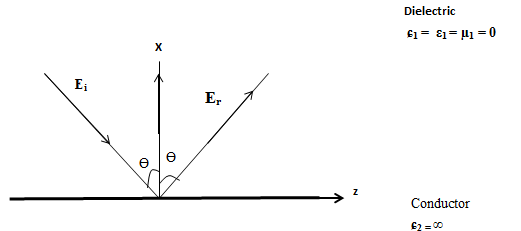
\includegraphics[width=1\linewidth]{plane}
	\caption{Conducting plane between two media}
\end{figure}
\\
 With reference to the figure above, we have a horizontal conductive plane which divides the medium into two parts. Below the plane is an ideal conductor with an infinite conductivity ($\sigma _2 =\infty$) and above the plane is the dielectric with conductivity $\sigma_1$, permeability $\mu _1$ and	permittivity $ \varepsilon _1 = 0 $. This plane or boundary can therefore be referred to as a \textbf{dielectric conductor boundary}.
 \\
 
 
 There can be no wave propagation in the conductor (conductive medium) due to its time varying fields, so the wave can only be propagated from the dielectric medium and then incident on the conductive plane/boundary.\\ Note that the time varying field of a conductor is zero.\\\\ As shown in figure 34.2, the wave \textbf{Ei}  is incident from the dielectric side making an angle $ \theta $ with the plane but it is not propagated to the
conductor side because of the infinite conductivity of the conductor,
hence no wave is transmitted. The wave Er is however reflected at an
angle $ \theta $ with the normal of the plane.\\ \textbf {From the law of reflection, the
angle of incidence is equal to the angle of reflection.}
\begin{figure}[h]
\centering
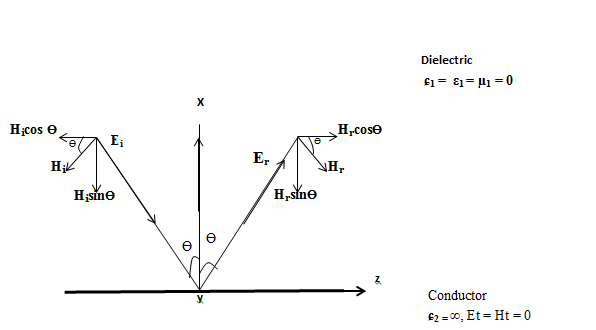
\includegraphics[width=1\linewidth]{fields}
\caption{Magnetic Field}
\end{figure}
\\

 Analyzing figure 34.3, we have two waves (a magnetic wave and an electric wave) for matching the boundary conditions, therefore, we can consider two polarizations;\\ 1. Perpendicular Polarization. \\ 2. Parallel Polarization. \\\\ Taking the perpendicular polarization, Ei and Er are oriented in the y
direction and by using pointing vector we get a direction for the magnetic fields Hi (incident magnetic field) and Hr (reflected magnetic field). We can resolve the magnetic field into two
components which are either \textbf{parallel} or \textbf{perpendicular} to the plane:
\\\\ $ H_isin\theta $ and $ H_rsin\theta $  are the normal(perpendicular) components to the plane. \\
$ H_icos\theta $ and $ H_rcos\theta $ are the tangential(parallel) components to the plane. \\\\
Since we are having a conducting boundary, there will be the presence of surface current, hence, we can either use the boundary conditions with appropriate surface current and the tangential component of the magnetic fields or use only the boundary condition without worrying about the surface current. Since there is no wave propagation in the conducting medium, the time varying fields $E_t$ and $H_t$ are zero, the boundary conditions now have to be satisfied by only the incident and reflected wave.
\\ Writing the expressions for the incident and reflected Electric and
Magnetic fields and taking the appropriate components of these fields
to satisfy the boundary conditions, we have that:
\\\\ The ratio of an electric and a magnetic field for both an incident and reflected wave is equal to the intrinsic impedance $\eta $.
\\\\ That is:
\\ $ \eta $ = intrinsic impedance
\\
\ $ \eta $ = $\sqrt{\mu_1 \varepsilon_1 }$
\\\ $\frac{E_r}{H_r} = \eta = \frac{E_i}{H_i}$
\\\\ \textbf{For Electric Field:}
\begin{align}
\bar{E}_i = E_i e^{-j\beta(-xcos\theta + zsin\theta)} \hat{y}  \end{align} 
\\ \begin{align}
\bar{E}_r =E_r  e^{-j\beta ( xcos\theta + zsin\theta)} \hat{y}
\end{align}  
\\ $\hat{y}$ signifies the field is in the y direction
\\\\ Where
\\ $\bar{E}_i$ = incident electric field
\\ $\bar{E}_r$ = reflected electric field
\\\ $E_i$, $E_r$ = amplitude
\\\ $e^{-j\beta}$ = phase function
\\\ $\beta$ = propagation constant = $\omega \sqrt{\mu_1\varepsilon_1}$ \\\\


\textbf{For Magnetic Field:}
 
\begin{align}
\bar{H}_i = (-H_i sin\theta \hat{x} - H_i cos\theta \hat{z}) e ^{-j\beta( -xcos\theta + zsin\theta)}
\end{align}
\\ \begin{align}
\bar{H}_r = (-H_r sin\theta \hat{x} + H_r cos\theta \hat{z}) e ^{-j\beta( xcos\theta + zsin\theta)}
\end{align}
\\ $\hat{x}$ signifies it's in the x direction  
\\ $\hat{z}$ signifies it's in the z direction\\\\

where
\\ $\bar{H}_i$= incident magnetic field
\\ $\bar{H}_r$= reflected magnetic field
\\ $H_i$, $H_r$ = amplitude
\\ \\\ As stated earlier $\frac{E_r}{H_r} = \eta = \frac{E_i}{H_i}$
\\\ Hence, $H_i = \frac{E_i}{\eta}$
\\\    and $H_r = \frac{E_r}{\eta}$
\\\ \\\ From the above, we can rewrite $H_i$ and $H_r$ in equations 34.3 and 34.4 in terms
of $E_i$ and $E_r$ respectively;
\\ \begin{align}
\bar{H}_i = - \frac{E_i}{\eta} (sin\theta \hat{x} + cos\theta \hat{z})e^{-j\beta (-xcos\theta + zsin\theta)}
\end{align}
\\ \begin{align}
\bar{H}_r =  \frac{E_r}{\eta} (-sin\theta \hat{x} + cos\theta \hat{z})e^{-j\beta (xcos\theta + zsin\theta)}
\end{align}
\\\\ So now that we have the expressions for the electric and magnetic
fields of the incident and the reflected waves, we need to obtain the
boundary conditions which are appropriate for the plane.\\ The boundary conditions are:
\\
1. The tangential component of the electric field should be continuous across the plane.
\\\\ 2. The normal component of the magnetic field should also be continuous across the plane.
\\\\ i.e
\\ $\bar{E}_tangential$ = continuous
\\ $\bar{H}_normal$ = continuous
\\\\ In the figure, we can see that the tangential component to the plane is
the electric field. At this point, if we equate x = 0 in equation 34.1 and 34.2, the sum of the two electric fields should be zero because
the fields are continuous and there are no fields in the conductive medium.
\\ \begin{align}
\bar{E} = (E_i + E_r) e^{-j\beta(zsin\theta) }\hat{y} = 0
\end{align}
\\\\ From here, we get the relation:
\\\ $E_i = - E_r$
\\\ i.e, $\frac{E_r}{E_i}$ = -1 \textbf{(reflection coefficient)}. \\\\
So in this case the electric field reflection coefficient is always equal
to -1. Similarly the sum of the two normal components of the
magnetic fields at x equal to 0 should be 0 because the normal
component are also continuous at the boundary.
\\\\ In transmission line analysis, the reflection coefficient is -1 for a \textbf{short	circuited load}. This means that the conducting boundary is identical to the short circuit condition on a transmission line. Therefore, the dielectric medium on which the wave is propagated is analogous to a
transmission line . When the electric wave reaches this ideal conductive boundary, it is completely
reflected from the boundary with a phase reversal (phase difference of
180 degrees). So this boundary essentially behaves like a short circuit
in the transmission line terminology. 
\\\\Now, we want to know the kind of field patterns that are created
when the electric field is completely reflected in the dielectric medium.
\\\\ \textbf{1. Electric field in the dielectric medium}
\\ Recall that $E_{i}$ = -$E_{r}$
\\ By superimposition of the two waves,
\\ $\bar{E}= \bar{E}_i + \bar{E}_r$
\\ Substitute $E_i$ = - $E_r$ and add equations 34.1 and 34.2
\\ \begin{align}
\bar{E}= \bar{E}_i e^{-j\beta zsin\theta} (e^{j\beta xcos\theta }- e^{-j\beta xcos\theta}) \hat{y}
\end{align}
\\\\ Recall that $e^{jx} - e^{-jx} = 2jsinx$
\\ From that analogy, 
\\ $e^{j\beta xcos\theta} - e^{-j\beta xcos\theta} = 2jsin\beta xcos\theta$
\\\\ Substituting into equation (34.8)
\\ \begin{align}
\bar{E}=2j \bar{E}_i sin(\beta xcos\theta) e^{-j\beta zsin\theta} \hat{y}
\end{align}
\\\\ From equation 34.9, we have the electric fields with sinusoidal
variation in the x direction and a phase term which is in the z direction. This means that the electric field has a \textbf{standing wave} behaviour in the x direction because the
function {sin({$\beta xcos\theta$})} does not have a phase but it is an amplitude
variation which is the nature of a complete standing wave. So equation 34.9 represents something like a standing
wave which is in the x direction and a traveling wave which is given
by this term \textbf{$e^{-j\beta zsin\theta}$} in the z direction.
The equation gives us a \textbf{standing wave} in x direction and a \textbf{traveling wave} in z direction. Therefore, the wave is a composite phenomenon
of the incident and the reflected wave making it a \textbf{complex wave}.\\ A complex wave is the combination of a standing wave which is in a
direction perpendicular to the plane/boundary and a traveling wave
which is in the direction of the plane.
\\\\ The same thing can be obtained for the magnetic fields when we
combine the incident and reflected magnetic fields. We therefore
would have an expression for a standing and traveling magnetic
wave.
\\\\ \textbf{2. Magnetic fields in the dielectric medium}
\\Taking two components of the magnetic field in the x and z direction
\textbf{Hx} and \textbf{Hz} respectively, and adding equations 34.5 and 34.6 we obtain:
\\\\
$H_x =[ \frac{-E_i}{\eta} (sin\theta \hat{x} + cos\theta \hat{z}) e^{-j\beta( -xcos\theta + zsin\theta)}] + 
\frac{E_r}{\eta} (-sin\theta \hat{x} + cos\theta \hat{z}) e^{-j\beta( xcos\theta + zsin\theta)}]$
\begin{align}
H_x = \frac{-E_i}{\eta}(sin\theta e^{j\beta( xcos\theta)} ) - \frac{E_r}{\eta}(sin\theta e^{-j\beta( xcos\theta)} (e^{-j\beta zsin\theta})
\end{align}
 Recall that $E_i$ = -$E_r$ and substituting into equation 34.10
\begin{align}
Hx = \frac{-E_i}{\eta}(sin\theta)( e^{j\beta( xcos\theta)} - e^{-j\beta( xcos\theta}) (e^{-j\beta zsin\theta})
\end{align}
 Recall that $e^{jx} - e^{-jx} = 2jsinx$ \\
From that analogy, $e^{j\beta xcos\theta} - e^{-j\beta xcos\theta} = 2jsin\beta xcos\theta$ \\\and substitute into
equation 34.11
 \begin{align}
Hx =  -2j \frac{E_i}{\eta}(sin\theta)( sin\beta xcos\theta) (e^{-j\beta zsin\theta})
\end{align} 
 The x component Hx has similar behaviour with the electric field.
That is, it has a standing wave component $(sin\beta xcos\theta)$ which is in x
direction and a traveling wave component $(e^{j\beta zsin\theta})$ in the z
direction.
\\\\ The same thing can be done for the z component of the magnetic field Hz.
\begin{align}
Hz = \frac{-E_i}{\eta}(cos\theta(e^{j\beta xcos\theta} + e^{-j\beta xcos\theta}) (e^{-j\beta zsin\theta})
\end{align}  
 Recall that $e^{jx} + e^{-jx} = 2cosx$
\\From that analogy, $e^{j\beta xcos \theta} - e^{-j\beta xcos\theta} = 2cos\beta xcos\theta$ \\ and substitute into equation 34.13
\begin{align}
Hz = \frac{-2E_i}{\eta}(cos\theta(cos\beta xcos\theta) (e^{-j \beta zsin\theta})
\end{align}
 From equation 34.14, we see that the z component of the magnetic field Hz has a standing wave component
$(cos\beta xcos\theta)$ and a traveling wave component $(e^{-j\beta zsin\theta})$. \\ So in general, the fields in the dielectric
medium are a combination of traveling wave and standing wave. \\ All of
these fields travel in the positive z direction (they travel along the plane) . However, note that the standing waves are in a direction
perpendicular to the interface.
\\\\ Now we can make some observations from the expressions which we
got for the electric and magnetic fields.
\\ First if we plot the amplitude of the electric field as a function of x
when x is equal to 0 then the amplitude is zero, therefore, the electric
field is zero. The same thing happens for the x component of the
magnetic field Hx, when x is equal to zero the magnetic field will be 0.
So whenever the electric field is zero the x component of the
magnetic field Hx is also zero. It can therefore be deduced that the
amplitude behaviour of Hx and electric field Ei is identical
as a function of x. And the magnetic field component of z is a cos
functions. That means it is shifted by a quarter cycles in the x
direction. So whenever Hx is zero Hz will be maximum and whenever Hx is
maximum Hz is zero.
\\\\ Plotting the amplitude of the electric and magnetic fields we get as follows:
\begin{figure}[h]
\centering
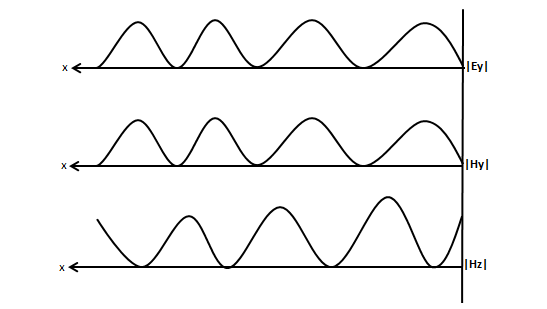
\includegraphics[width=1\linewidth]{amplitude.png}
\caption{Amplitude of electric and magnetic fields}
\end{figure}
\\\\ Referring to the figure 34.4, we have a boundary consisting of an electric field Ey, a magnetic field Hx for the x
component and a magnetic field on the z component Hz. We can see
that both fields Ey and Hx are exactly identical in behaviour whereas
the magnetic field on the z component Hz is shifted with respect to a
cos function. The Ey and Hx patterns are aligned in space but the Hz
pattern is shifted by a quarter cycle. So wherever Hx is maximum, Hz
is 0 and vice versa. Since Hz which is the tangential component (along the plane) is not
zero, there will therefore be surface currents on the plane and
the magnitude of the surface current will be equal to the tangential
component of the magnetic field. When the wave is incident on
the conducting boundary, the surface currents are going to get reduced
on this surface which is due to the tangential component of the
magnetic field. Also, the normal component of the magnetic field and the tangential component of the electric field will be zero.
\\ With reference to the expression for the electric field in equation 34.9,
the electric field is zero when x is equal to zero and it will also be zero whenever this quantity $(\beta xcos\theta)$ is a multiple of $\pi$. This means that
Ey will be 0 when $(\beta xcos\theta)$ is a multiple of $\pi$.
i.e Ey will be zero when:
\\ $(\beta xcos\theta) = m\pi$     where m is an integer (0,1,2 ?)
\\ $ x = \frac{m\pi}{\beta xcos\theta}$   
\\ but $\beta = \frac{2\pi}{\lambda}$ \\where $\lambda$ is the wavelength in the dielectric medium
\\ $x =\frac{m\pi}{ \frac{2\pi}{\lambda (cos\theta)}} $
\\ $x = \frac{m\lambda}{2cos\theta}$ 
\\\\ So at this distance x from the plane, the electric field will be 0. This is however dependent 
on this distance x and the angle where the wave is launched
on the plane.\\ There are multiple
planes here in which the electric field is zero and since the electric field and the x component of the magnetic field
Hx have the same behaviour in those planes, both quantities will be zero
but Hz will be maximum. If we go by a quarter cycle away, we will
see that the Hz will be 0 and these quantities Ey and Hx will be
maximum.
\\ Now, we know that the wave is traveling along the z direction so
there must be a power flow in that direction. This essentially gives us
the pointing vector in the z direction. Note that there is no net power
flow in the x direction.\\ Given that we have a conducting boundary, there will be no power flow into the boundary. So whatever power is incident on the boundary is reflected back to the source medium. The wave is
incident in the x direction and has a component of propagation in the
direction. The wave which is incident normal to the interface is
completely reflected, hence, a standing wave is created. Since there is
no net power flow in the x direction, there is however a reactive
power in the x direction.
Given a conducting boundary, the boundary can be used to guide a
wave of energy along it, hence, the conducting boundary has the
capability of guiding electromagnetic energy. When a wave is launched at an arbitrary angle, the net power flow is always along the
surface of the boundary interface. This is the principle used in making
a waveguide. \\ So in a wave guiding structure, the conducting
boundaries are used so that the electromagnetic energy is guided along the
boundaries.
\\\\ Later in this book, we will look at a more realizable structure called a \textbf{parallel plane waveguide}.